% Vorbereitung: Vorbereitungsaufgaben bearbeiten
% Versuchsaufbau: Verwendete Apparatur, Beschreibung Funktionsweise/Nutzen mit Skizze/Foto
\section{Durchführung}
\label{sec:durchführung}

In der Abbildung ist der verwendete Aufbau für den Versuch zur Bestimmung der Reichweite von $\alpha$-Teilchen zu sehen.
\begin{figure}[H]
	\centering
    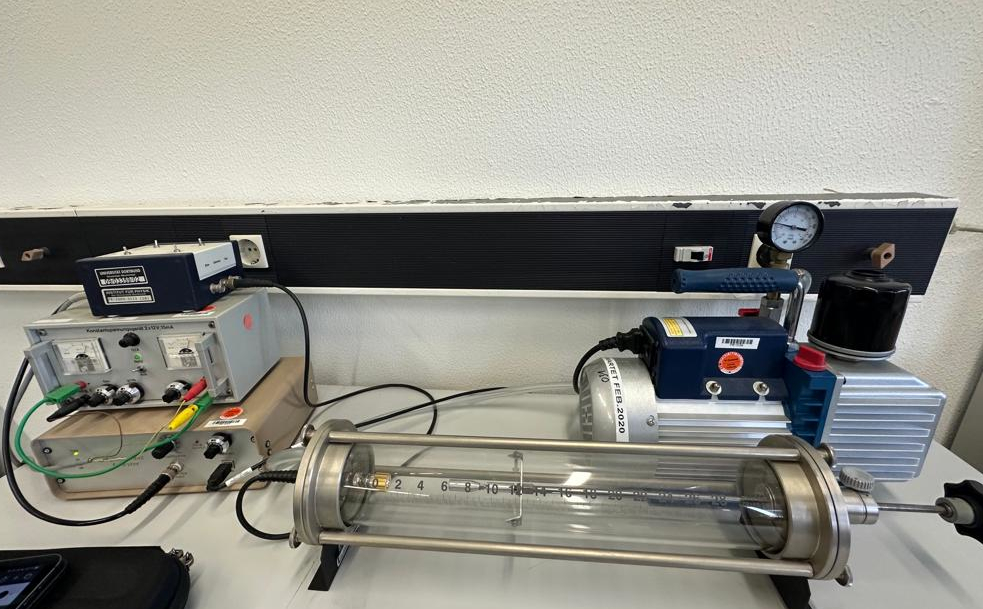
\includegraphics[width=0.75\linewidth]{content/grafik/aufbau.jpg}
    \caption{Der Versuchsaufbau zur Bestimmung der Reichweite von $\alpha$-Teilchen.}
    \label{fig:aufbau}
\end{figure}
In einem evakuierten Glaszylinder befindet sich das $\alpha$-Präparat un dein Detektor. Mittels einer Vakuumpumpe
wird der Glaszylinder evakuiert, sodass zum Start der ersten Messung ein Druck von $\SI{0}{mbar}$ herrscht.
Als Strahlungsquelle wird ein Am-Präparat verwendet. Dieses zerfällt mit einer Halbwertszeit von $ \symup{T}_{1/2} = 459 a$ in
\begin{equation*}
    \ce{^{241}_95Am -> ^{237}_93N + ^4_2He^{++}} .
\end{equation*}
Das Präparat befindet sich an einem verschiebbaren Regler, sodass es möglich ist einen Abstand $x$ zum Detektor
einzustellen. Als Detektor wird ein Hableiter-sperrschichtzähler verwendet.

Bevor der Versuch durchgeführt werden kann, muss der Aufbau und dessen Verkabelung überprüft werden
